%%%%%%%%%%%%%%%%%%%%%%%%%%%%%%%%%%%%%%%%%%%%%%%%%%%%%%%%%%%%%%%%%%%%%%%%%%%%%%%%
%2345678901234567890123456789012345678901234567890123456789012345678901234567890
%        1         2         3         4         5         6         7         8
%% PP_Report.tex
%% V1.4
%% 2015/11/30
%% by Rui Santos Cruz
%% This is a skeleton file using PPIEEEtran.cls
%% (requires PPIEEEtran.cls) 
% !TEX root = ./main.tex
%%%%%%%%%%%%%%%%%%%%%%%%%%%%%%%%%%%%%%%%%%%%%%%%%%%%%%%%%%%%%%%%%%%%%%%%%%%%%%%%

\documentclass[a4paper,12pt,journal,twoside,compsoc]{PPIEEEtran}

% -----------------------------------------------------------------------------
% The Preamble document contains all the necessary Packages for typesetting
% Modify it to suit your needs
% -----------------------------------------------------------------------------
%%%%%%%%%%%%%%%%%%%%%%%%%%%%%%%%%%%%%%%%%%%%%%%%%%%%%%%%%%%%%%%%%%%%%%%%%%%%%%%%
%2345678901234567890123456789012345678901234567890123456789012345678901234567890
%        1         2         3         4         5         6         7         8
% Required Packages and commands
% --> Please Choose the MAIN LANGUAGE for the document in package BABEL (below)
% --> Please Choose the TYPE OF REPORT for the document in \ReportType (below)
% !TEX root = ./main.tex
% PP_Report_Preamble.tex
% V1.4
% 2015/11/30
% by Rui Santos Cruz
%%%%%%%%%%%%%%%%%%%%%%%%%%%%%%%%%%%%%%%%%%%%%%%%%%%%%%%%%%%%%%%%%%%%%%%%%%%%%%%%
%
% *** INPUT LANGUAGE PACKAGES ***

\usepackage[main=english]{babel}
\usepackage[utf8]{inputenc}
\usepackage{iflang}

% *** DEFINE THE TYPE OF REPORT ***
\newcommand*{\ReportType}{learning}% Uncomment line for Learning Report
%\newcommand*{\ReportType}{activity}% Uncomment line for Activity Report

% *** ACRONYM PACKAGES ***
% Put definition of Acronyms at the end of the document
\usepackage[printonlyused,nolist]{acronym}

% *** CITATION PACKAGES ***
\usepackage{cite}

% *** GRAPHICS RELATED PACKAGES ***
\usepackage[pdftex]{graphicx}
\DeclareGraphicsExtensions{.pdf,.jpeg,.png}

% *** MATH PACKAGES ***
\usepackage[cmex10]{amsmath}

% *** SPECIALIZED LIST PACKAGES ***
\usepackage{algorithmic}

% *** ALIGNMENT PACKAGES ***
\usepackage{array}

% *** SUBFIGURE PACKAGES ***
\usepackage[caption=false,font=normalsize,labelfont=sf,textfont=sf]{subfig}

% *** FLOAT PACKAGES ***
\usepackage{fixltx2e}

% *** PDF, URL AND HYPERLINK PACKAGES ***
\usepackage{url}

% *** BACKGROUND Material ***
\usepackage{eso-pic}
\usepackage[
  contents={},
  opacity=1,
  scale=1,
  color=blue!90
  ]{background}
  
% *** CONDITIONALS ***
\usepackage{ifthen}

% DEFINE COMMAND FOR: Report Type depending on language
\newcommand{\tlangRepActivity}{\IfLanguageName{english}{Activity Report}{Relatório de Atividade}}
\newcommand{\tlangRepLearning}{\IfLanguageName{english}{Learnings Report}{Relatório de Aprendizagens}}
%%%%%%%%%%%%%%%%%%%%%%%%%%%%%%%%%%%%%%%%%%%%%%%%%%%%%%%%%%%%%%%%%%%%%%%%%%%%%%%%
% DEFINE COMMAND FOR: Report Scoring Table Type
\newcommand{\lrScore}%
{\setlength{\unitlength}{1mm}{% % selecting unit length 
\fontfamily{phv}\selectfont
\begin{picture}(171.6,20) % picture environment with the size (dimensions)
% 32 length units wide, and 15 units high.
\setlength\fboxsep{0pt}
% Left Set with grading Scores
\put(0,0){\fcolorbox{gray}{gray!20}{%
          \framebox(15,4)[l]{\scriptsize{0.2-Weak}}}}
\put(0,4){\fcolorbox{gray}{gray!20}{%
          \framebox(15,4)[l]{\scriptsize{0.4-Fair}}}}
\put(0,8){\fcolorbox{gray}{gray!20}{%
          \framebox(15,4)[l]{\scriptsize{0.6-Good}}}}
\put(0,12){\fcolorbox{gray}{gray!20}{%
           \framebox(15,4)[l]{\scriptsize{0.8-V.Good}}}}
\put(0,16){\fcolorbox{gray}{gray!20}{%
           \framebox(15,4)[l]{\scriptsize{1.0-Excel}}}}
% Left+1 Set with Learning Rubrics
\put(16,0){\fcolorbox{cyan}{white}{%
          \framebox(12,12)[c]{\footnotesize{ }}}}
\put(28,0){\fcolorbox{cyan}{white}{%
          \framebox(12,12)[c]{\footnotesize{ }}}}          
\put(40,0){\fcolorbox{cyan}{white}{%
          \framebox(12,12)[c]{\footnotesize{ }}}}
\put(52,0){\fcolorbox{cyan}{white}{%
          \framebox(12,12)[c]{\footnotesize{ }}}}
\put(64,0){\fcolorbox{cyan}{white}{%
          \framebox(12,12)[c]{\footnotesize{ }}}}
\put(16,12){\fcolorbox{cyan}{white}{%
          \framebox(12,4)[c]{\tiny{Intro$\times 2$}}}}
\put(28,12){\fcolorbox{cyan}{white}{%
          \framebox(12,4)[c]{\tiny{Motiv$\times 2$}}}}          
\put(40,12){\fcolorbox{cyan}{white}{%
          \framebox(12,4)[c]{\tiny{Skills$\times 6$}}}}
\put(52,12){\fcolorbox{cyan}{white}{%
          \framebox(12,4)[c]{\tiny{Reflect$\times 6$}}}}
\put(64,12){\fcolorbox{cyan}{white}{%
          \framebox(12,4)[c]{\tiny{Sugg$\times 2$}}}}
\put(16,16){\fcolorbox{cyan}{cyan!20}{%
          \framebox(60,4)[c]{\footnotesize{LEARNINGS}}}}
% Middle Set with Document Rubrics
\put(77,0){\fcolorbox{green}{white}{%
          \framebox(12,12)[c]{\footnotesize{ }}}}
\put(89,0){\fcolorbox{green}{white}{%
          \framebox(12,12)[c]{\footnotesize{ }}}}
\put(101,0){\fcolorbox{green}{white}{%
          \framebox(12,12)[c]{\footnotesize{ }}}}
\put(113,0){\fcolorbox{green}{white}{%
          \framebox(12,12)[c]{\footnotesize{ }}}}
\put(125,0){\fcolorbox{green}{white}{%
          \framebox(12,12)[c]{\footnotesize{ }}}}
\put(137,0){\fcolorbox{green}{white}{%
          \framebox(12,12)[c]{\footnotesize{ }}}}
\put(77,12){\fcolorbox{green}{white}{%
          \framebox(12,4)[c]{\tiny{Struct $\times .25$}}}}
\put(89,12){\fcolorbox{green}{white}{%
          \framebox(12,4)[c]{\tiny{Ortog$\times .25$}}}}          
\put(101,12){\fcolorbox{green}{white}{%
          \framebox(12,4)[c]{\tiny{Gram$\times .25$}}}}
\put(113,12){\fcolorbox{green}{white}{%
          \framebox(12,4)[c]{\tiny{Form $\times .25$}}}}
\put(125,12){\fcolorbox{green}{white}{%
          \framebox(12,4)[c]{\tiny{Abstr $\times .5$}}}}
\put(137,12){\fcolorbox{green}{white}{%
          \framebox(12,4)[c]{\tiny{Concl $\times .5$}}}}
\put(77,16){\fcolorbox{green}{green!20}{%
          \framebox(72,4)[c]{\footnotesize{DOCUMENT}}}}
% Right Set with Penalties
\put(150,0){\fcolorbox{red}{white}{%
          \framebox(10,12)[c]{\footnotesize{ }}}}
\put(160,0){\fcolorbox{red}{white}{%
          \framebox(10,12)[c]{\footnotesize{ }}}}
\put(170,0){\fcolorbox{red}{white}{%
          \framebox(10,12)[c]{\footnotesize{ }}}}
\put(150,12){\fcolorbox{red}{white}{%
          \framebox(10,4)[c]{\tiny{Titles $\times .5$}}}}
\put(160,12){\fcolorbox{red}{white}{%
          \framebox(10,4)[c]{\tiny{Files $\times .5$}}}}
\put(170,12){\fcolorbox{red}{white}{%
          \framebox(10,4)[c]{\tiny{IDs $\times .5$}}}}
\put(150,16){\fcolorbox{red}{red!20}{%
          \framebox(30,4)[c]{\footnotesize{PENALTY}}}}
\end{picture}
}}
%%%%%%%%%%%%%%%%%%%%%%%%%%%%%%%%%%%%%%%%%%%%%%%%%%%%%%%%%%%%%%%%%%%%%%%%%%%%%%%%
%\newcommand{\arScore}%
\newcommand{\arScore}%
{\setlength{\unitlength}{1mm}{% % selecting unit length 
\fontfamily{phv}\selectfont
\begin{picture}(171.6,20) % picture environment with the size (dimensions)
% 32 length units wide, and 15 units high.
\setlength\fboxsep{0pt}
% Left Set with grading Scores
\put(0,0){\fcolorbox{gray}{gray!20}{%
          \framebox(15,4)[l]{\scriptsize{0.2-Weak}}}}
\put(0,4){\fcolorbox{gray}{gray!20}{%
          \framebox(15,4)[l]{\scriptsize{0.4-Fair}}}}
\put(0,8){\fcolorbox{gray}{gray!20}{%
          \framebox(15,4)[l]{\scriptsize{0.6-Good}}}}
\put(0,12){\fcolorbox{gray}{gray!20}{%
           \framebox(15,4)[l]{\scriptsize{0.8-V.Good}}}}
\put(0,16){\fcolorbox{gray}{gray!20}{%
           \framebox(15,4)[l]{\scriptsize{1.0-Excel}}}}
% Left+1 Set with Activity Rubrics
\put(16,0){\fcolorbox{yellow}{white}{%
          \framebox(12,12)[c]{\footnotesize{ }}}}
\put(28,0){\fcolorbox{yellow}{white}{%
          \framebox(12,12)[c]{\footnotesize{ }}}}          
\put(40,0){\fcolorbox{yellow}{white}{%
          \framebox(12,12)[c]{\footnotesize{ }}}}
\put(52,0){\fcolorbox{yellow}{white}{%
          \framebox(12,12)[c]{\footnotesize{ }}}}
\put(64,0){\fcolorbox{yellow}{white}{%
          \framebox(12,12)[c]{\footnotesize{ }}}}
\put(16,12){\fcolorbox{yellow}{white}{%
          \framebox(12,4)[c]{\tiny{Intro$\times 2$}}}}
\put(28,12){\fcolorbox{yellow}{white}{%
          \framebox(12,4)[c]{\tiny{Object$\times 2$}}}}          
\put(40,12){\fcolorbox{yellow}{white}{%
          \framebox(12,4)[c]{\tiny{Plan$\times 4$}}}}
\put(52,12){\fcolorbox{yellow}{white}{%
          \framebox(12,4)[c]{\tiny{Exec$\times 6$}}}}
\put(64,12){\fcolorbox{yellow}{white}{%
          \framebox(12,4)[c]{\tiny{Result$\times 4$}}}}
\put(16,16){\fcolorbox{yellow}{yellow!20}{%
          \framebox(60,4)[c]{\footnotesize{ACTIVITY}}}}
% Middle Set with Document Rubrics
\put(77,0){\fcolorbox{green}{white}{%
          \framebox(12,12)[c]{\footnotesize{ }}}}
\put(89,0){\fcolorbox{green}{white}{%
          \framebox(12,12)[c]{\footnotesize{ }}}}
\put(101,0){\fcolorbox{green}{white}{%
          \framebox(12,12)[c]{\footnotesize{ }}}}
\put(113,0){\fcolorbox{green}{white}{%
          \framebox(12,12)[c]{\footnotesize{ }}}}
\put(125,0){\fcolorbox{green}{white}{%
          \framebox(12,12)[c]{\footnotesize{ }}}}
\put(137,0){\fcolorbox{green}{white}{%
          \framebox(12,12)[c]{\footnotesize{ }}}}
\put(77,12){\fcolorbox{green}{white}{%
          \framebox(12,4)[c]{\tiny{Struct $\times .25$}}}}
\put(89,12){\fcolorbox{green}{white}{%
          \framebox(12,4)[c]{\tiny{Ortog$\times .25$}}}}          
\put(101,12){\fcolorbox{green}{white}{%
          \framebox(12,4)[c]{\tiny{Gram$\times .25$}}}}
\put(113,12){\fcolorbox{green}{white}{%
          \framebox(12,4)[c]{\tiny{Form $\times .25$}}}}
\put(125,12){\fcolorbox{green}{white}{%
          \framebox(12,4)[c]{\tiny{Abstr $\times .5$}}}}
\put(137,12){\fcolorbox{green}{white}{%
          \framebox(12,4)[c]{\tiny{Concl $\times .5$}}}}
\put(77,16){\fcolorbox{green}{green!20}{%
          \framebox(72,4)[c]{\footnotesize{DOCUMENT}}}}
% Right Set with Penalties
\put(150,0){\fcolorbox{red}{white}{%
          \framebox(10,12)[c]{\footnotesize{ }}}}
\put(160,0){\fcolorbox{red}{white}{%
          \framebox(10,12)[c]{\footnotesize{ }}}}
\put(170,0){\fcolorbox{red}{white}{%
          \framebox(10,12)[c]{\footnotesize{ }}}}
\put(150,12){\fcolorbox{red}{white}{%
          \framebox(10,4)[c]{\tiny{Titles $\times .5$}}}}
\put(160,12){\fcolorbox{red}{white}{%
          \framebox(10,4)[c]{\tiny{Files $\times .5$}}}}
\put(170,12){\fcolorbox{red}{white}{%
          \framebox(10,4)[c]{\tiny{IDs $\times .5$}}}}
\put(150,16){\fcolorbox{red}{red!20}{%
          \framebox(30,4)[c]{\footnotesize{PENALTY}}}}
\end{picture}
}}

% DEFINE COMMAND FOR: Printing Scoring Table Type
\newcommand\BackgroundPic{%
\put(-15,12){%
\parbox[b][\paperheight]{\paperwidth}{%
\vfill
\centering
\ifthenelse{\equal{\ReportType}{activity}}{\arScore}{\lrScore}}}}
% Printing the Scoring Table
\AddToShipoutPicture*{\BackgroundPic}

% Print Vertical Identifications on even and odd pages
\AddEverypageHook{%
  \ifthenelse{\isodd{\value{page}}}%
  {\backgroundsetup{
    angle=90,
    position={-0.1\textwidth,-1.055\textheight},
    contents={\tiny{PP-2015 V1.4}}
    }% Odd Pages
  }%
  {\backgroundsetup{
    angle=90,
    position={0.97\textwidth,-1.05\textheight},%
    contents={\ifthenelse{\equal{\ReportType}{activity}}{%
              \tiny{\tlangRepActivity}}{\tiny{\tlangRepLearning}}}
    }% Even Pages
  }%
  \BgMaterial}
% correct bad hyphenation here
\hyphenation{op-tical net-works semi-conduc-tor}
%%%%%%%%%%%%%%%%%%%%%%%%%%%%%%%%%%%%%%%%%%%%%%%%%%%%%%%%%%%%%%%%%%%%%%%%%%%%%%%%
%2345678901234567890123456789012345678901234567890123456789012345678901234567890
%        1         2         3         4         5         6         7         8
\begin{document}
%%%%%%%%%%%%%%%%%%%%%%%%%%%%%%%%%%%%%%%%%%%%%%%%%%%%%%%%%%%%%%%%%%%%%%%%%%%%%%%%
%2345678901234567890123456789012345678901234567890123456789012345678901234567890
%        1         2         3         4         5         6         7         8
%% PP_Report_Cover.tex
%% V1.4
%% 2015/11/30
%% by Rui Santos Cruz
% !TEX root = ./main.tex
%%%%%%%%%%%%%%%%%%%%%%%%%%%%%%%%%%%%%%%%%%%%%%%%%%%%%%%%%%%%%%%%%%%%%%%%%%%%%%%%
% paper title
% can use linebreaks \\ within to get better formatting as desired
% Do not put math or special symbols in the title.
\title{Por2folios Platform}
%%%%%%%%%%%%%%%%%%%%%%%%%%%%%%%%%%%%%%%%%%%%%%%%%%%%%%%%%%%%%%%%%%%%%%%%%%%%%%%%
% Author names
%
% note positions of commas and nonbreaking spaces ( ~ ) LaTeX will not break
% a structure at a ~ so this keeps an author's name from being broken across
% two lines.
% use \thanks{} to gain access to the first footnote area
% a separate \thanks must be used for each paragraph.
%
%\IEEEcompsocitemizethanks is a special \thanks that produces the bulleted
% lists for "first footnote" author affiliations. 
% Use \IEEEcompsocthanksitem which works much like \item
% for each affiliation group.
\author{Francisco~Maria~Calisto% <-this % stops a space
% Change the Course Name 
% note: need leading \protect in front of \\ to get a newline within \thanks as
% \\ is fragile and will error, could use \hfil\break instead.
\IEEEcompsocitemizethanks{
\IEEEcompsocthanksitem Bruno~Cardoso, nr. 72619,\protect\\ 
E-mail: bruno.f.cardoso@tecnico.ulisboa.pt,
\IEEEcompsocthanksitem Francisco~Maria~Calisto, nr. 70916,\protect\\
E-mail: francisco.calisto@tecnico.ulisboa.pt,
\IEEEcompsocthanksitem Nuno~Sousa, nr. 73216,\protect\\
E-mail: nuno.g.sousa@tecnico.ulisboa.pt,\protect\\
Instituto Superior Técnico, Universidade de Lisboa.\protect\\}% <-this % stops an unwanted space}% <-this % stops an unwanted space
\thanks{Manuscrito recebido em Julho 24, 2016.}
}
%%%%%%%%%%%%%%%%%%%%%%%%%%%%%%%%%%%%%%%%%%%%%%%%%%%%%%%%%%%%%%%%%%%%%%%%%%%%%%%%
% The paper headers
\markboth{Por2folios}%
% for a single student
%{Surname}% : for a single student 
% for a Group Report 
{Surname \MakeLowercase{\textit{et al.}}}% : for a Group Report 
%
% The only time the second header will appear is for the odd numbered pages
% after the title page when using the twoside option.
%%%%%%%%%%%%%%%%%%%%%%%%%%%%%%%%%%%%%%%%%%%%%%%%%%%%%%%%%%%%%%%%%%%%%%%%%%%%%%%%
% Prints in Subtitle the type of Report
% PLEASE DO NOT CHANGE THIS SECTION
\IEEEspecialpapernotice{%
\ifthenelse{\equal{\ReportType}{activity}}{%
\tlangRepActivity}{\tlangRepLearning}
}
%%%%%%%%%%%%%%%%%%%%%%%%%%%%%%%%%%%%%%%%%%%%%%%%%%%%%%%%%%%%%%%%%%%%%%%%%%%%%%%%
%%%%%%%%%%%%%%%%%%%%%%%%%%%%%%%%%%%%%%%%%%%%%%%%%%%%%%%%%%%%%%%%%%%%%%%%%%%%%%%%
% The paper Abstract and Keywords
\IEEEtitleabstractindextext{%
\begin{abstract}
The goal of this report is to describe and highlight every stage on the development of a platform called Po2folios, developed during the semester. The main goal on this platform is to showcase every project and report developed during previous editions of the Portfolio III and IV classes
\end{abstract}
%
\begin{IEEEkeywords}
Wordpress, Por2folios, projects, reports, PPIV, PPIII.
\end{IEEEkeywords}}
%%%%%%%%%%%%%%%%%%%%%%%%%%%%%%%%%%%%%%%%%%%%%%%%%%%%%%%%%%%%%%%%%%%%%%%%%%%%%%%%
% make the title area
\maketitle

\IEEEdisplaynontitleabstractindextext
\IEEEpeerreviewmaketitle
%%%%%%%%%%%%%%%%%%%%%%%%%%%%%%%%%%%%%%%%%%%%%%%%%%%%%%%%%%%%%%%%%%%%%%%%%%%%%%%%
%%%%%%%%%%%%%%%%%%%%%%%%%%%%%%%%%%%%%%%%%%%%%%%%%%%%%%%%%%%%%%%%%%%%%%%%%%%%%%%%
\section{Introduction}
% The very first letter is a 2 line initial drop letter followed
% by the rest of the first word in caps (small caps for compsoc).
% 
% form to use if the first word consists of a single letter:
% \IEEEPARstart{A}{demo} file is ....
% 
% Here we have the typical use of a "E" for an initial drop letter
% and "STE" in caps to complete the first word.
\IEEEPARstart{T}{he} development of this platform was time restricted, as we were already experienced in web development. With this in mind, we were careful not to commit to features that would exceed this time limit, and, managed to complete version 1.0 of the platform.
%%%%%%%%%%%%%%%%%%%%%%%%%%%%%%%%%%%%%%%%%%%%%%%%%%%%%%%%%%%%%%%%%%%%%%%%%%%%%%%%
\section{early experience}
During my first 3 years in Computer Science, I learned that there is a set of rules as to "how to interact with our client". For a start, there is the need to perfectly understand the requirements a platform must have, and, from previous work experience, I did learn that, despite the developer and client think alike, what they are really thinking is remotely different from each other.
To give an example, when the client asks for a web repository, my main idea is to develop some sort of an FTP server where an interface allows access to several people involved in the project. Yet, as in this case, the goal is not to simply store files, but to showcase them. As this is a recurring situation on the IT World, there is a need to establish a communication channel between the client and the development team. For this, we decided to report every situation internally, by email, and also by scheduling a meeting with our client.

\section{The First Steps}
For the first three to four weeks, I was aware that there was a platform to be developed, and my basic idea was to develop something that included a good interface, so that our colleagues had no difficulty in accessing the platform to add content, but also to allow every web visitor to easily access the previous developed projects on this class.

It was only after the first meeting with the team, along with Professor Rui Cruz, that we were able to establish what was to be developed. This included the platform layout, some required functionalities, an interface for the content managers, and also some general aspects.


\section{Team Work}
As explained before, the key element for a successful team work is communication. With this in mind, Calisto and I maintained a team work channel for this project. This included a Facebook Conversation, and a couple of presencial meetings at Técnico. 
As Calisto is more of an interface developer, and I prefer to give support on server side, it was decided that I would be in charge of the server setup. I do remind at this point that our Virtual Machine was Vanilla at this stage, only with Ubuntu 12 installed.
After choosing our working platform, my job was essentially to prepare the VM to receive the WordPress Suite. At every stage, Calisto was up to date with the development, and could begin its interface development.

\section{Progress}
I consider that this was a very successful project. For a start, we started working as soon as possible, and that gave us time to carefully thing about each aspect of this project. Looking back at the semester, we did everything we decided on our meetings. This included a fully functional platform, our webserver, domain and the tags feature.
	For this to happen, we have reserved 2 to 3 hours per week to develop this project. Most of the work happened after our Thursday theoretical lesson, and usually ended up by 2 AM.
	The main challenge here was to successfully setup the apache server, and to install an easy to use server management service. Installing WebMin ( as suggested by our teacher) was one of the best decision we did, as it allows us to connect to the server using an HTTP protocol, and a specific port. Although this may not be the most secure connection ever, as the SSL certificate was not up to date, to access the server, we do require login credentials, and, it is up to each user's responsibility not to eavesdrop their own credentials.
	After successfully setting up WebMin, simple tasks such as adding a user, or installing a new module on the server, or even redirecting to a specific incoming address is easily done online, anywhere. We are used to do this using a Secure Shell, but, to keep this platform user friendly, we have decided to follow this approach.
	In the middle of this project, Nuno, our colleague, joined this project, and helped us develop the rest of the platform. He was also essencial for the release of our beta platform. The final TAGS feature, where one can associate one or more keywords to a portfolio project, was developed by Nuno. He was also responsible for adding the older keywords from previous years.
	
	
\section{Overall}
Overall, this project was very fullfilling, as it helped us develop our technical skills regarding interfaces, server setup and maintenance. It was also responsible for the development of our soft skills, as we used them a lot during this project. For example, problem solving got easier when using these new soft skills.
As a group, we all did a great job, as we maintained communication, and every decision was made as a group, with the consent of everyone.
We did divide the work among the group, taking advantage of each member's skills on each feature of our platform.
The final version of this platform is fully functional, with all the features we agreed on during the beginning of the semester. There is a front-end and a back-office, where we are able to create new users, and to add content. We can also grant admin access to these new users, and make them content managers.

%%%%%%%%%%%%%%%%%%%%%%%%%%%%%%%%%%%%%%%%%%%%%%%%%%%%%%%%%%%%%%%%%%%%%%%%%%%%%%%%
\section{\IfLanguageName{english}{Conclusion}{Conclusão}}
In conclusion, developing the Por2folios platfrom was only possible with the work of all the members involved, our team, and professor Rui Cruz. By working together, we were able to add new features every week, and, although we did not had any close deadlines, the development was time consistent.

Overall, this project was very enriching, and it made me grow as a professional. By cooperating and with the ease of communication, my integration on the team was very successful, and even when our new team member Nuno joined us, the team was able to continue as before.

The platform is available on its final address por2folios.tecnico.ulisboa.pt.
We will continue maintaining this server, and, hopefully, start adding the older projects soon.

%%%%%%%%%%%%%%%%%%%%%%%%%%%%%%%%%%%%%%%%%%%%%%%%%%%%%%%%%%%%%%%%%%%%%%%%%%%%%%%%
% use section* for acknowledgement
\ifCLASSOPTIONcompsoc
  % The Computer Society usually uses the plural form
  \section*{\IfLanguageName{english}{Acknowledgments}{Agradecimentos}} % Acknowledgments
\else
  % regular IEEE prefers the singular form
  \section*{Acknowledgment}
\fi

The author would like to thank teacher Rui Cruz, for all the support and availability from day 1. Also, to thank the Técnico IT Department, for providing a Virtual Machine for this project, and setting up the right "domain" for the server.
Lastly, I would like to show appreciation for my colleagues, as they were always there ready to assist, and to make this a successful project.
There will be more work next semester, and I do count on them to continue developing this project, by adding new features.

%%%%%%%%%%%%%%%%%%%%%%%%%%%%%%%%%%%%%%%%%%%%%%%%%%%%%%%%%%%%%%%%%%%%%%%%%%%%%%%%
% biography section
% 
\begin{IEEEbiography}[{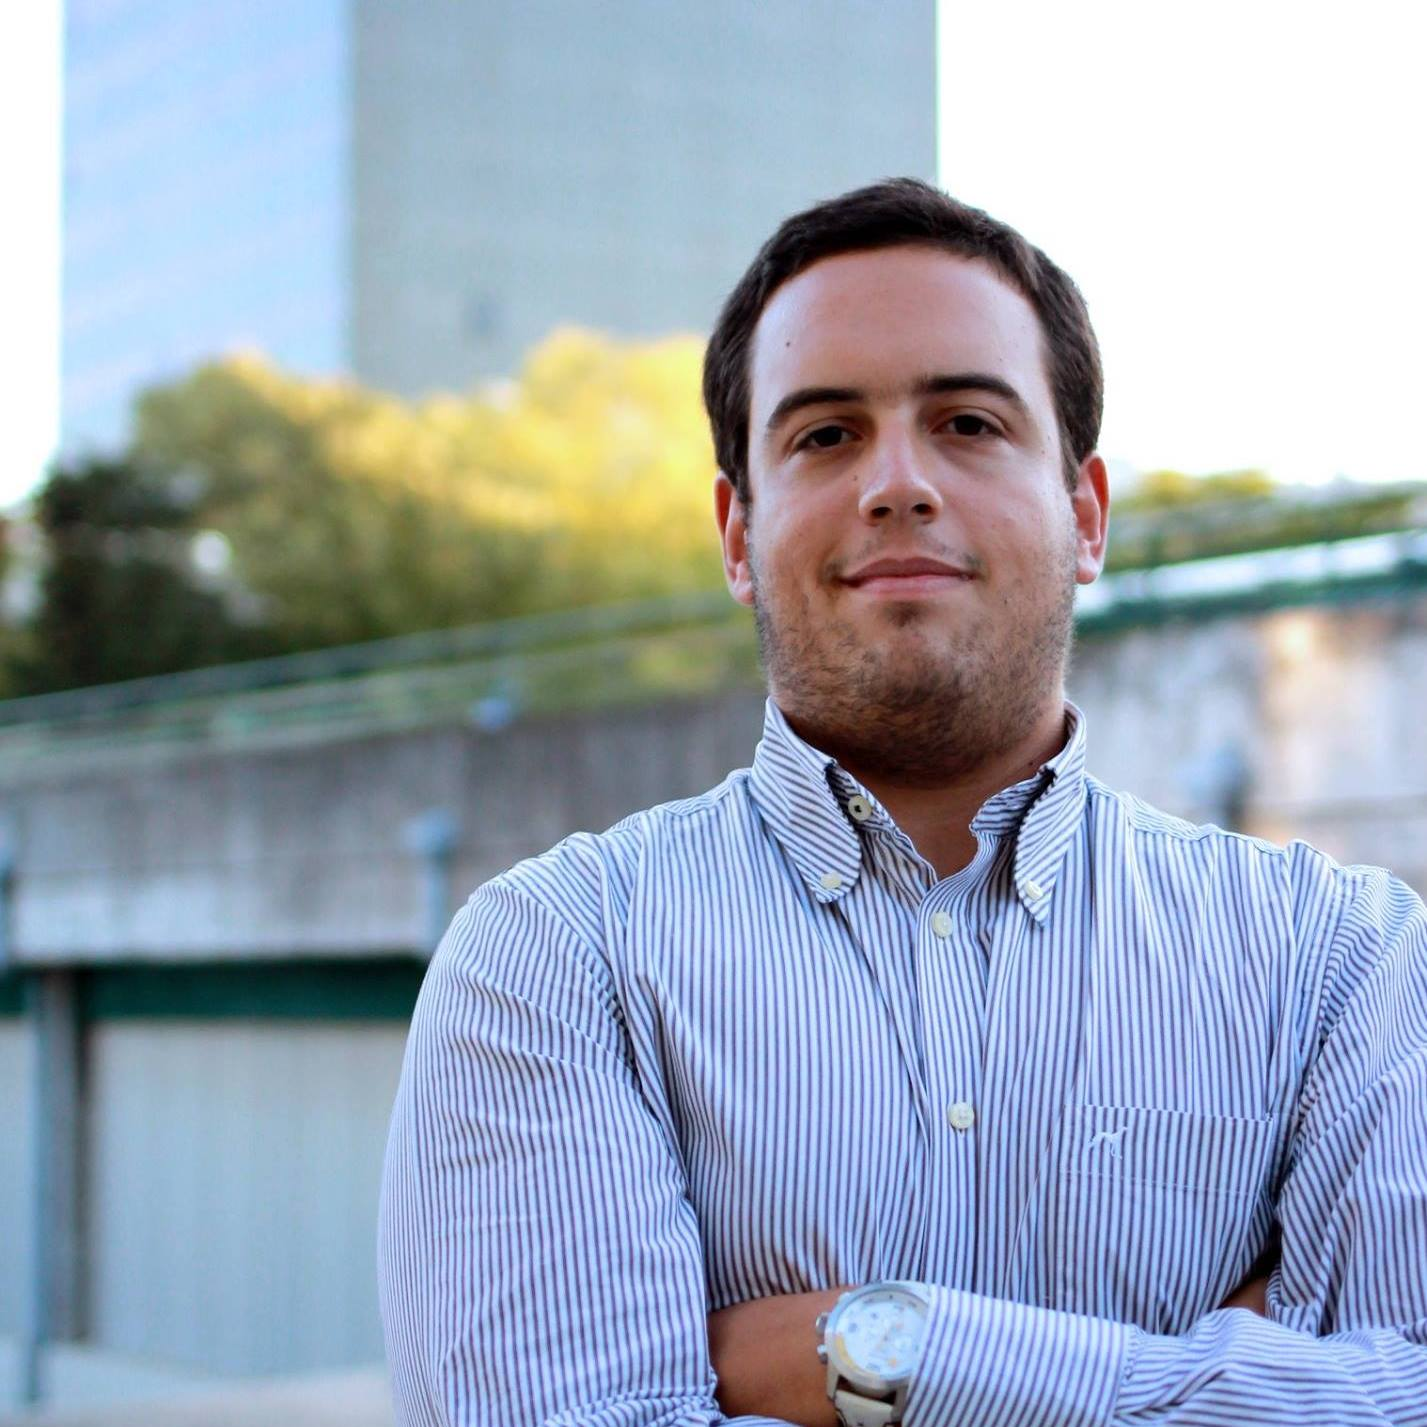
\includegraphics[width=1in,height=1.25in,clip,keepaspectratio]{bruno.png}}]{Bruno Cardoso}
Here I am. I am pursuing my Engineering studies at \ac{IST}. Starting my masters in Interaction and Visualization, and also on business systems. On my "spare" time, I am also developing a project at INESC-ID, at VIMMI.
\end{IEEEbiography}

%%%%%%%%%%%%%%%%%%%%%%%%%%%%%%%%%%%%%%%%%%%%%%%%%%%%%%%%%%%%%%%%%%%%%%%%%%%%%%%%


% *** DEFINITION OF ACRONYMS ***
	\acrodef{CPU}{Central Processing Unit}
	\acrodef{GUI}{Graphical User Interface}
	\acrodef{HTTP}{Hypertext Transfer Protocol}
	\acrodef{IST}{Instituto Superior Técnico}	
	\acrodef{LAN}{Local Area Network}
	\acrodef{PC}{Personal Computer}
	\acrodef{URL}{Uniform Resource Locator}
	\acrodef{VoD}{Video-on-demand}
	\acrodefplural{VoD}[VoDs]{Videos-on-demand}
	\acrodef{VoIP}{Voice over IP}
	\acrodef{WAN}{Wide Area Network}
	\acrodef{WLAN}{Wireless Local Area Network}
	\acrodef{WWAN}{Wireless Wide Area Network}
	\acrodef{WWW}{World Wide Web}
	
% that's all folks
\end{document}